\subsection{Análisis de tiempos en función de los parámetros de entrada}
En esta sección analizaremos de manera experimental como varían los tiempos de ejecución de los algoritmos descriptos al variar el largo y el ancho de la matriz y la cantidad de sanguijuelas del sistema.

\subsubsection{Ancho en función del tiempo}
Para comenzar, tomaremos un parabrisas con 50 sanguijuelas tal que estas solo afecten un punto de la discretización, y para una granularidad fija de $1.0$ iremos variando el largo del parabrisas. De esta manera, comenzaremos con un parabrisas de $50 \times 50$ luego uno de $60 \times 50$ y asi aumentando de manera lineal ambos parámetros hasta llegar a un parabrisas de $100 \times 50$. Resolveremos cada uno de estos sistemas utilizando ambos metodos implementados (Gauss y Descomposición LU). Los resultados obtenidos pueden verse en el siguente gráfico:

\begin{center}
 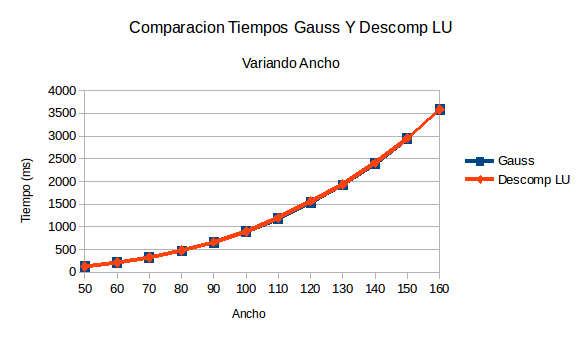
\includegraphics[width=400pt]{imagenes/testeo/anchoGauss.png}
\end{center}

Sabemos que al aumentar el largo del parabrisas de manera lineal, aumentará también de manera lineal el número de ecuaciones en nuestra matriz de resolución. Lo que puede observarse en este gráfico es que con un aumento lineal del largo del parabrisas, el tiempo de ejecución aumenta de manera semi-lineal. Esto era esperable ya que sabemos que tanto el gauss como la descomposición LU tienen una complejidad igual a $O(n*p^2)$, y dado que en nuestro modelado, utilizamos el largo del parabrisas para definir el tamaño de la banda en la matriz de resolución (es decir $p$), resulta lógico que al aumentar el largo, se obtuviera un aumento casi cuadrático en el tiempo de ejecución.
\\
Además, en este gráfico se pueden observar que tanto los tiempos de la factorización LU como la de gauss son similares.
\\
Ahora, utilizando la misma familia de parabrisas descripta anteriormente, veremos como se comportan ambos métodos de salvación.

Dado que nos aseguramos que cada sanguijuela solo toque un punto de la discretización, nos aseguramos que podremos utilizar el metodo de Sherman-Morrison. Para estos algoritmos, el gráfico es el siguiente:
\\
\begin{center}
 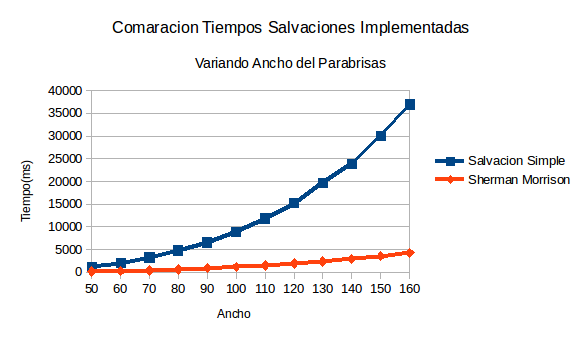
\includegraphics[width=400pt]{imagenes/testeo/anchoSalv.png}
\end{center}

Como era de esperar, el algoritmo que utiliza la optimización de Sherman-Morrison es mucho más rapido y escala mejor que la versión simple que debe calcular todo el sistema desde cero, ademas el Sherman-Morrison realiza operaciones sobre vectores y escalares haciendo la diferencia en el modo de comparacion respecto al método anterior.

\subsubsection{Largo en función del tiempo}
Ahora, analizaremos que sucede dejando fijo el ancho y variando el largo del parabrisas. Las condiciones son las mismas que en el test anterior, solo que ahora el ancho permaence constante igual a $50$ y se varía el largo de $50$ a $100$.

\begin{center}
 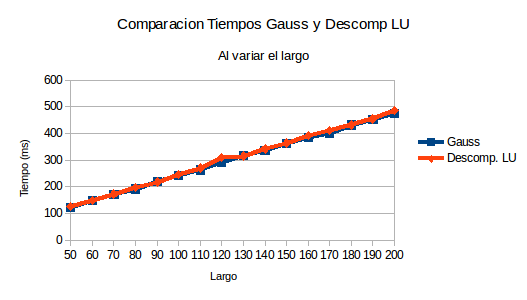
\includegraphics[width=400pt]{imagenes/testeo/largoGauss.png}
\end{center}

En este caso los tiempos de ejecución crecen de manera estrictamente lineal. Esto se debe que a diferencia del ancho, el largo no interviene en el cálculo del tamaño de la banda de la matriz de resolución. Luego, al aumentar el largo, solo aumenta la cantidad de incógnitas $n$.
\\
Aplicando el mismo experimento para los dos métodos de salvación:

\begin{center}
 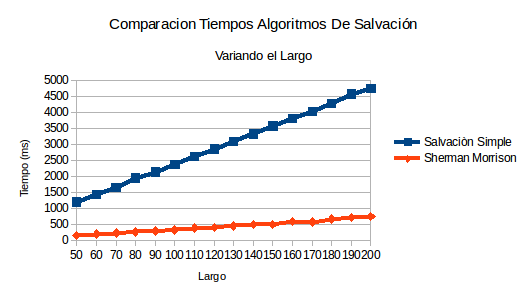
\includegraphics[width=400pt]{imagenes/testeo/largoSalv.png}
\end{center}

Al igual que lo dicho en la sección anterior, aqui también se pueden ver las ventajas de utilizar Sherman-Morrison. Además en este caso también puede apreciarse el comportamiento lineal de ambos algoritmos al variar el largo del sistema.

\subsubsection{Cantidad de sanguijuelas en función del tiempo}
Para el siguente experimento, variamos la cantidad de sanguijuelas y dejamos fija tanto la granularidad como el largo y el ancho del parabrisas. Nuevamente, por una cuestión de simplicidad, las sanguijuelas solo afectan un punto de la discretización. Para el experimento tomamos un parabrisas de $100 \times 100$, una granularidad igual a $1.0$, y variamos la cantidad de sanguijuelas desde $10$ hasta $100$. Resolviendo el sistema con el algoritmo de Gauss y Descomposicion LU, se obtuvo el siguiente grafico.

\begin{center}
 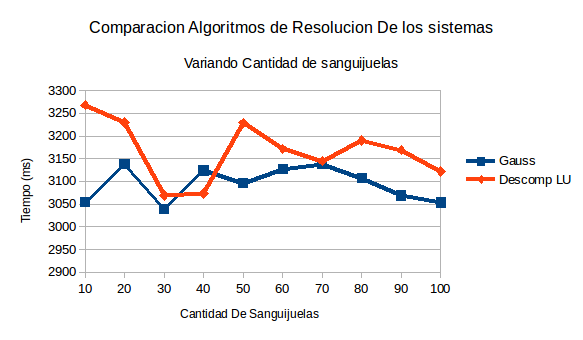
\includegraphics[width=400pt]{imagenes/testeo/sangGauss.png}
\end{center}

Como vemos, no se muestra ningún patrón visible al modificar la cantidad de sanguijuelas del sistema. Esto es porque la cantidad de incógnitas continúa siendo la misma.
\\
Ahora, utilizando el mismo experimento para el problema del último disparo, resolviendo este parabrisas con ambos algoritmos, se obtuvo este gráfico:

\begin{center}
 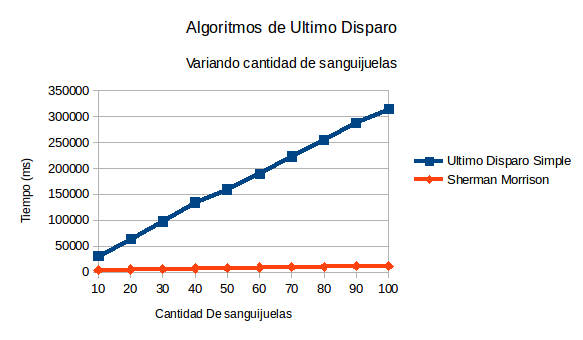
\includegraphics[width=400pt]{imagenes/testeo/sangSalv.png}
\end{center}

En este gráfico se puede apreciar como si bien ambos algoritmos dependen de manera lineal de la cantidad de sanguijuelas, el algoritmo de Sherman-Morrison presenta una mejor velocidad y una mejor escalabilidad.

\subsubsection{Granularidad en función del tiempo}
Por ultimo, veremos como afecta variar la granularidad de la discretización para ver como se ve afectada la performance. Para este experimento se dejan fijos el largo y el ancho, iguales a $100$, la cantidad de sanguijuelas iguales a $5$ y se varía la granularidad desde $0.4$ hasta $0.9$, aumentando de $0.1$ en cada paso. Se obtiene lo siguiente:

\begin{center}
 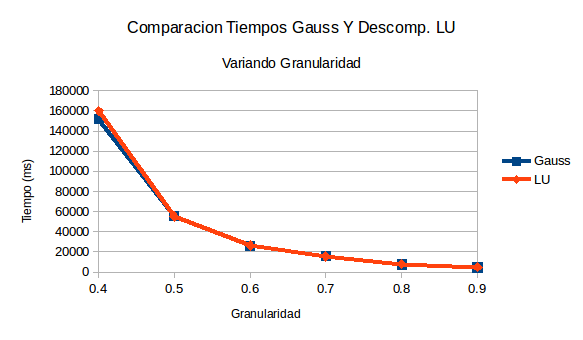
\includegraphics[width=400pt]{imagenes/testeo/granuGauss.png}
\end{center}

En el gráfico puede observarse que una disminución lineal de la granularidad produce un aumento cuadrático en el tiempo de ejecución. Esto se debe a que tanto la cantidad de filas y la cantidad de columnas viene dado por el largo/ancho del parabrisas, dividido por granularidad. Dado que el tamaño de nuestra matriz de resolución del problema viene dado por $\text{Cantidad De filas} \times \text{Cantidad De Columnas}$ esto será lo mismo que  $(\text{Largo} \times \text{Ancho}) / \text{granularidad}^2$. En esta fórmula puede verse claramente que disminuir la granularidad de manera lineal produce un aumento cuadrático en el número de incógnitas de nuestro problema.

\subsection{Análisis de temperatura en función de las discretizaciones}
Partiendo de la base de que un aumento en la granularidad permite una mejor representación de las sanguijuelas (son circulos), notamos que con este aumento y mejora en la representación, el problema discreto parece al menos perceptualmente para el ojo humano, volverse continuo. Teniendo en cuenta esta información, queda claro como una baja granularidad impacta directamente sobre la precisión de los resultados (a expensas, como vimos con anterioridad, de los tiempos de cómputo).
\\
En el siguiente experimento, mostramos como varían los resultados al variar la granularidad:
\begin{itemize}
 \item Matriz $20 \times 20$, granularidad 2.\\
  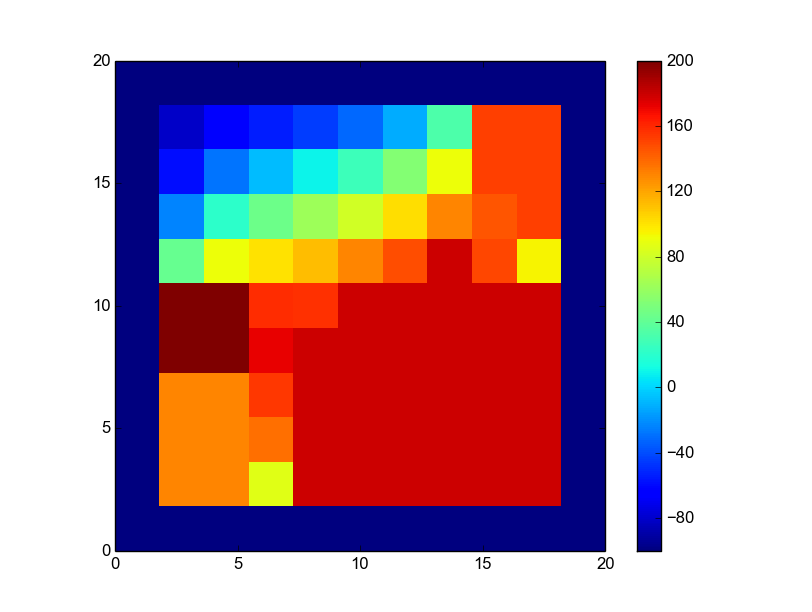
\includegraphics[width=400pt]{imagenes/imagen11.png}

 \item Matriz $20 \times 20$, granularidad 1.\\
  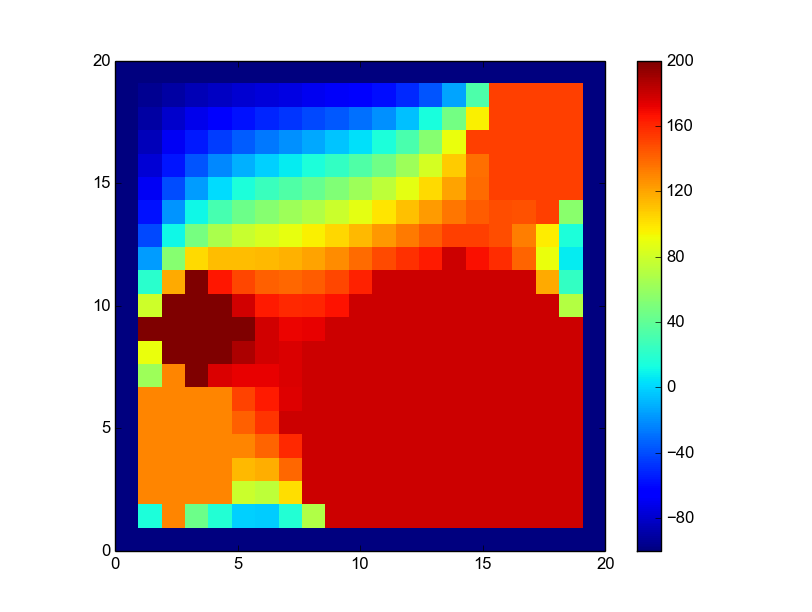
\includegraphics[width=400pt]{imagenes/imagen21.png}

 \item Matriz $20 \times 20$, granularidad 0,5.\\
  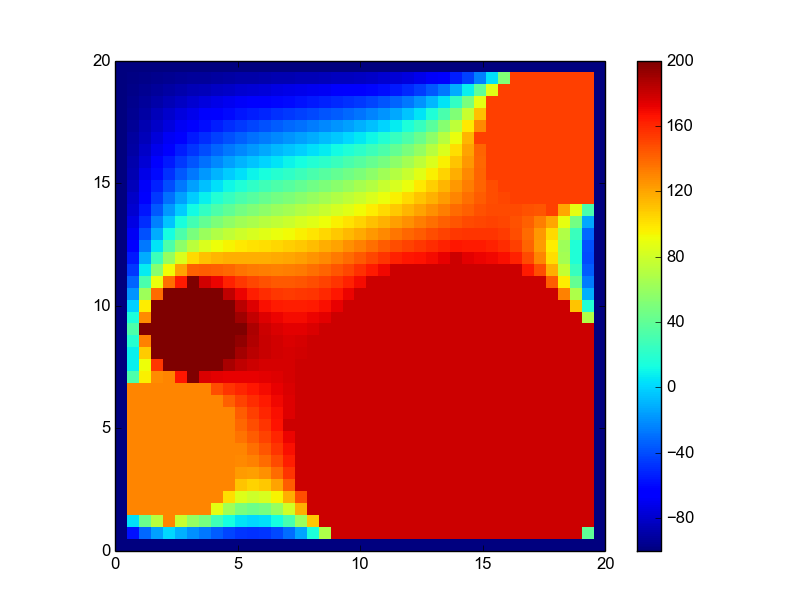
\includegraphics[width=400pt]{imagenes/imagen31.png}
  
   \item Matriz $20 \times 20$, granularidad 0,1.\\
  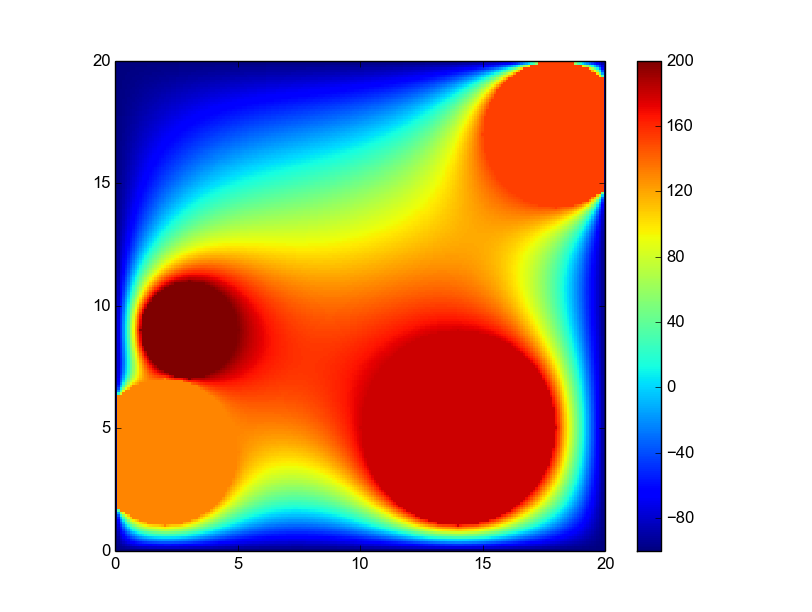
\includegraphics[width=400pt]{imagenes/imagen41.png}
\end{itemize}

Puede notarse a simple vista que una granularidad más pequeña produce resultados que aproximan más exactamente a lo que uno creería es el resultado real de la ecuación diferencial de la que partimos en la introducción, ya que para una granularidad de $2$ pueden verse grandes bloques discretos, pero para la discretización de $0.1$ puede verse que estos bloques desaparecen y puede notarse una cierta \"suavidad\"' en el resultado obtenido, propio de una función continua y derivable. Esto puede verse en el gráfico ya que la tonalidad va oscureciendo hasta llegar a rojo generando circulos grandes, de ser chicos estaríamos viendo un pico en la función y no sería derivable.
\\
Además, al disminuir la granularidad, está claro que la cantidad de incógnitas cercanas al punto crítico aumenta, por lo que, en caso de no poder tomarlo de manera exacta, al menos podremos tomar un vecino muy próximo a este por lo que tendemos a pensar que la presición del resultado tambien aumentará por ese lado.
